% !TeX TS-program = lualatex
% use lualatex because of academicons

\documentclass[11pt,a4paper,onecolumn]{article}

% -- begin Packages

\usepackage[utf8]{inputenc}
\usepackage[T1]{fontenc}
\usepackage{amsmath}
\usepackage{amsfonts}
\usepackage{amssymb}
\usepackage{graphicx}
\usepackage[left=3.00cm, right=3.00cm, top=3.00cm, bottom=3.00cm]{geometry}

\usepackage{fancyhdr}

%\usepackage{lipsum}
\usepackage{wrapfig}
\usepackage{fontawesome}
\usepackage{academicons}
\usepackage{enumitem}

\usepackage[english]{babel}

% --
% for including individual full refecenre in text
% --
\usepackage[square,numbers]{natbib}
\usepackage{bibentry}
\nobibliography*
% --

\usepackage[colorlinks=true, 
linkcolor=blue, 
urlcolor=blue,
citecolor=blue
]{hyperref}

%\usepackage[backend=bibtex, style=alphabetic, sorting=ydnt]{biblatex}
%\addbibresource{papers.bib}


\frenchspacing % Better looking spacings after periods
%\pagestyle{empty}           % No pagenumbers/headers/footers

% The command above will ensure that if two files are encountered with the same basename 
% but different extensions (for example image.eps, image.pdf, image.jpeg and image.png), 
% then the .eps version will be used first, .pdf version will be used second, .jpeg will be used
% third and finnaly the .png will be used in the absence of other versions
\DeclareGraphicsExtensions{.eps,.pdf,.jpeg,.png,.jpg}

% -- end Packages

% -- begin Macros

\newcommand{\FundingEntry}[9]{
	% agency, language, title, language, title, id, grant name, amount, period
	\noindent #1, Title (#2): \textit{#3}, Title (#4): \textit{#5}, ID: #6, Research grant: #7, R\$ #8, #9.}

\newcommand{\ThesisEntry}[9]{
	% type (MSc or PhD), language, title, language, title, student, institution, year conclusion
	\noindent \textbf{[#1]} Title (#2): \textit{#3}, Title (#4): \textit{#5}, Author: #6, \textsl{#7} (#8). \sloppy{\textbf{\texttt{doi:}}~ \href{https://doi.org/#9}{\texttt{#9}}}}
	
\newcommand{\ThesisEntryTEDE}[9]{
	% type (MSc or PhD), language, title, language, title, student, institution, year conclusion
	\noindent \textbf{[#1]} Title (#2): \textit{#3}, Title (#4): \textit{#5}, Author: #6, \textsl{#7} (#8). \sloppy{\textbf{\texttt{url:}}~ \href{http://sistede.on.br:8080/jspui/handle/tede/#9}{\texttt{sistede.on.br:8080/jspui/handle/tede/{#9}}}}}

\newcommand{\Student}[5]{
	% #1 level (MSc or PhD), #2 main or co supervisor, #3 name, since #4, #5 institution
	\noindent \textbf{#1} #2 supervisor of #3 \hfill 
	\parbox{0.1\textwidth}{\raggedleft since~#4} \\
	\noindent\textsl{#5}}

% -- end Macros

\begin{document}
	
\section*{CONTACT INFORMATION}

% -- begin Section content 
{

% Insert the picture
\begin{wrapfigure}{r}{-0.10\textwidth} 
	\centering
	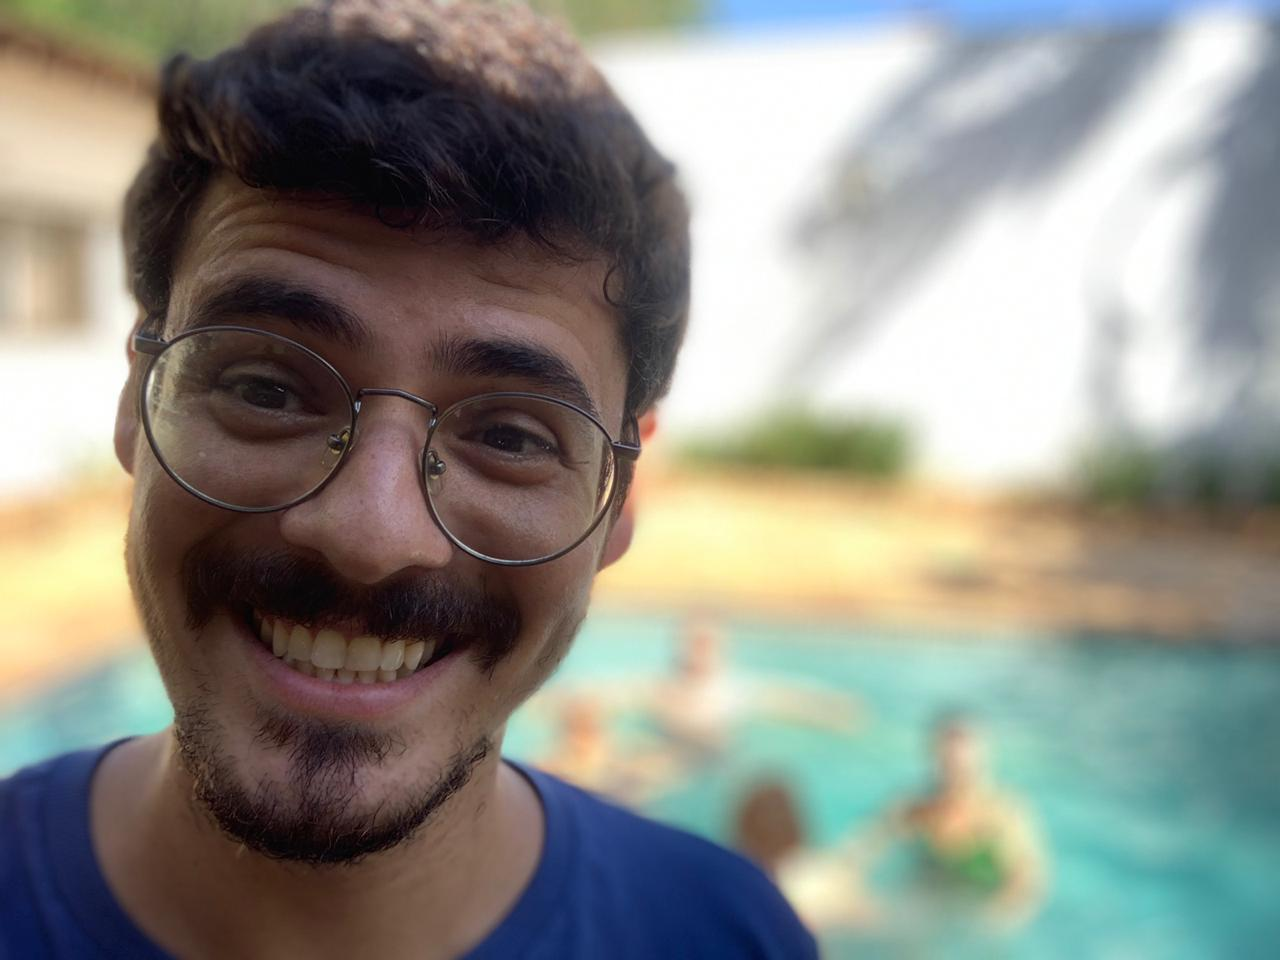
\includegraphics[width=0.40\textwidth,angle=-90]{foto.jpg}
\end{wrapfigure}

\parbox{0.03\textwidth}{\faUser} \textbf{Vanderlei C. Oliveira Jr.}\\
\parbox{0.03\textwidth}{\faInstitution} \href{https://www.gov.br/observatorio/pt-br}{\textit{Observatório Nacional}}\\
\parbox{0.03\textwidth}{\faMapMarker} \href{https://g.page/observatorionacional?share}{\textit{Rio de Janeiro - RJ, Brazil}}\\
\parbox{0.03\textwidth}{\faEnvelope} \href{mailto:vanderlei@on.br}{\texttt{vanderlei@on.br}}\\
\parbox{0.03\textwidth}{\faGithub} \href{https://github.com/birocoles}{\footnotesize \texttt{github.com/birocoles}}\\\\
\parbox{0.03\textwidth}{\faGroup} \href{https://www.pinga-lab.org/people/oliveira-jr.html}{\footnotesize \texttt{pinga-lab.org/people/oliveira-jr}}\\
\parbox{0.03\textwidth}{\aiLattes} \href{https://lattes.cnpq.br/4332841435949533}{\footnotesize \texttt{lattes.cnpq.br/4332841435949533}}\\
\parbox{0.03\textwidth}{\aiOrcid} \href{https://orcid.org/0000-0002-6338-4086}{\footnotesize \texttt{orcid.org/0000-0002-6338-4086}}\\
\parbox{0.03\textwidth}{\aiPublonsSquare} \href{https://publons.com/researcher/1454914/oliveira-jr-v-c/}{\footnotesize  \texttt{publons.com/researcher/1454914/oliveira-jr-v-c}}\\
\parbox{0.03\textwidth}{\aiImpactstory} \href{https://impactstory.org/u/0000-0002-6338-4086}{\footnotesize \texttt{impactstory.org/u/0000-0002-6338-4086}}\\
\parbox{0.03\textwidth}{\aiResearchGateSquare} \href{https://www.researchgate.net/profile/Vanderlei-Oliveira-Jr}{\footnotesize \texttt{researchgate.net/profile/Vanderlei-Oliveira-Jr}}\\
\parbox{0.03\textwidth}{\aiFigshare} \href{https://figshare.com/authors/Vanderlei_C_Oliveira_Jr/387579}{\footnotesize \texttt{figshare.com/authors/Vanderlei{\_}C{\_}Oliveira{\_}Jr}}\\

} % -- end Section content

\bigskip \hrule

\section*{OVERVIEW}

Full Professor at the geophysics department of Observat\'{o}rio Nacional, Brazil.
Specialist in numerical methods for processing and interpreting potential 
fields (gravity and magnetic).

\bigskip \hrule

\section*{APPOINTMENTS}

\noindent \textbf{Full Professor of Geophysics} \\
\noindent \textsl{Observat\'{o}rio Nacional, Brazil} \hfill \parbox{0.1\textwidth}{\raggedleft 2020--present} \vspace{0.5\baselineskip} \\
\noindent \textbf{Associate Professor of Geophysics} \\
\noindent \textsl{Observat\'{o}rio Nacional, Brazil} \hfill \parbox{0.1\textwidth}{\raggedleft 2016--2020} \vspace{0.5\baselineskip} \\
\noindent \textbf{Assistant Professor of Geophysics} \\
\noindent \textsl{Observat\'{o}rio Nacional, Brazil} \hfill \parbox{0.1\textwidth}{\raggedleft 2013--2016} \vspace{0.5\baselineskip} \\

\bigskip \hrule

\section*{RESEARCH INTERESTS}

% command [leftmargin=*], from enumitem package, removes the default indent of itemize
\begin{itemize}[leftmargin=*]

\item{\textbf{Equivalent layer technique:} computationally efficient methods for processing and interpreting large potential field data sets.}

\item{\textbf{Inversion of gravity and/or magnetic data:} methods to invert gravity and/or magnetic data for the purpose of estimating the position and shape of geological bodies.}

\item{\textbf{Magnetization of geological bodies:} methods for estimating the magnetization direction of geological bodies by using land and airborne magnetic data.}

\item{\textbf{Magnetization of rock samples:} methods for estimating the magnetization distribution within rock samples by using scanning magnetic microscopy data.}

\item{\textbf{Magnetic modeling of geological bodies:} methods for computing the demagnetizing field within geological bodies having high susceptibility.}

\item{\textbf{Regional characterization of gravity field:} computationally efficient methods for representing the regional gravity field by combining different data sets.}

\item{\textbf{Regional characterization of the crustal magnetic field:} computationally efficient methods for representing the crustal field by combining different data sets.}
		
\end{itemize}

\bigskip \hrule

\section*{EDUCATION}

\medskip

\noindent \textbf{\Large PhD Geophysics} \\
\noindent \href{https://www.gov.br/observatorio/pt-br}{\textsl{Observat\'{o}rio Nacional, Brazil}} \hfill \parbox{0.25\textwidth}{\raggedleft Dec/2010 -- Jan/2013} \vspace{0.3\baselineskip} \\
\noindent \textbf{Title (portuguese):} \textit{Processamento e invers\~{a}o de dados de campos potenciais: novas abordagens} \\
\noindent \textbf{Title (english):} \textit{Processing and inversion of potential field data: new approaches} \\
\noindent \textbf{Advisor:} \href{https://orcid.org/0000-0002-9767-6044}{Dr. Val{\'e}ria C. F. Barbosa} \\
\noindent \textbf{Description:} This work presents two new methodologies for processing and interpreting potential field data. The first one is the Polynomial Equivalent Layer, which is a cost-effective method for processing large potential-field data sets via the equivalent-layer technique. The second is a non-linear method for inverting gravity-gradient data to estimate the shape of isolated 3-D geological bodies. \\
\noindent \texttt{\textbf{doi:}}\href{https://doi.org/10.6084/m9.figshare.20334651.v1}{\texttt{ 10.6084/m9.figshare.20334651.v1}} \\

\medskip

\noindent \textbf{\Large MSc Geophysics} \\
\noindent \href{https://www.gov.br/observatorio/pt-br}{\textsl{Observat\'{o}rio Nacional, Brazil}} \hfill \parbox{0.25\textwidth}{\raggedleft Mar/2009 -- Nov/2010} \vspace{0.3\baselineskip} \\
\noindent \textbf{Title (portuguese):} \textit{Invers\~{a}o gravim\'{e}trica radial por camadas para a reconstru\c{c}\~{a}o de corpos geol\'{o}gicos 3D} \\
\noindent \textbf{Title (english):} \textit{Radial gravity inversion by layers for retrieving 3D geological bodies} \\
\noindent \textbf{Advisor:} \href{https://orcid.org/0000-0002-9767-6044}{Dr. Val{\'e}ria C. F. Barbosa} \\
\noindent \textbf{Description:} This work presents a gravity-inversion method for estimating the geometry of a 3D source. The subsurface region containing the geologic source is discretized into an ensemble of vertically juxtaposed prisms. By estimating the coordinates of the horizontal section of each prism, the method retrieves a set of polygonal horizontal sections representing depth slices of the 3D gravity source. \\
\noindent \texttt{\textbf{doi:}}\href{https://doi.org/10.6084/m9.figshare.20334531.v1}{ \texttt{10.6084/m9.figshare.20334531.v1}} \\

\medskip

\noindent \textbf{\Large BSc Geophysics} \\
\noindent \href{https://www.iag.usp.br/international/}{\textsl{University of S\~{a}o Paulo, Brazil}} \hfill \parbox{0.25\textwidth}{\raggedleft Mar/2004 -- Dec/2008} \vspace{0.3\baselineskip} \\
\noindent \textbf{Title (portuguese):} \textit{Modelagem gravim\'{e}trica 3D da borda norte da Bacia do Paran\'{a}} \\
\noindent \textbf{Title (english):} \textit{3D gravity modelling of the northern border of the Paran\'{a} basin} \\
\noindent \textbf{Advisor:} \href{https://orcid.org/0000-0003-4329-1787}{Dr. Y{\'a}ra R. Marangoni} \\
\noindent \textbf{Description:} This work presents a geological model of the northern border of the Paran\'{a} basin obtained from gravity data. \\

\pagebreak \hrule


\section*{PEER-REVIEWED JOURNAL PAPERS (\href{https://orcid.org/0000-0002-6338-4086}{ORCID})}


% command [leftmargin=*], from enumitem package, removes the default indent of itemize
\begin{enumerate}[leftmargin=*, label=\textbf{(\arabic*)}]
	\item \bibentry{piauilino_etal2024}
	\item \bibentry{oliveirajr_etal2023}
	\item \bibentry{arelaro_etal2023}
	\item \bibentry{takahashi_etal2022}
	\item \bibentry{barbosa_etal2022}
	\item \bibentry{gonzalez_etal2022}
	\item \bibentry{vital_etal2021}
	\item \bibentry{melo_etal2021}
	\item \bibentry{hidalgo-gato_etal2021}
	\item \bibentry{takahashi_etal2020}
	\item \bibentry{reis_etal2020}
	\item \bibentry{maurya_etal2020}
	\item \bibentry{bastos_oliveirajr2020}
	\item \bibentry{araujo_etal2019_materials}
	\item \bibentry{araujo_etal2019_sensors}
	\item \bibentry{takahashi_oliveirajr2017}
	\item \bibentry{siqueira_etal_2017}
	\item \bibentry{reis_etal2016}
	\item \bibentry{oliveirajr_etal_2015}
	\item \bibentry{uieda_etal2014}
	\item \bibentry{oliveirajr_etal_2013}
	\item \bibentry{melo_etal2013}
	\item \bibentry{oliveirajr_barbosa2013}
	\item \bibentry{oliveirajr_etal2011}
\end{enumerate}

\bigskip \hrule

\section*{INTERNATIONAL CONFERENCES}

% command [leftmargin=*], from enumitem package, removes the default indent of itemize
\begin{enumerate}[leftmargin=*, label=\textbf{(\arabic*)}]
	\item \bibentry{seg_2020_eqlayer_remanent}
	\item \bibentry{seg_2020_fast_mag_eqlayer}
	\item \bibentry{seg_2020_conv_eqlayer}
	\item \bibentry{seg_2019_amplitude}
	\item \bibentry{sbgf_2019_amplitude}
	\item \bibentry{seg_2019_eql_magdir}
	\item \bibentry{sbgf_2019_gradgrav}
	\item \bibentry{seg_2019_gradgrav}
	\item \bibentry{seg_2019_radial_mag}
	\item \bibentry{aseg_2019_radial_mag}
	\item \bibentry{sbgf_2019_4Dgrav}
	\item \bibentry{eage_2017_fast_eqlayer}
	\item \bibentry{latinmag_2017}
	\item \bibentry{sbgf_2016_elipsoid}
	\item \bibentry{agu_fallmeeting_2016a}
	\item \bibentry{agu_fallmeeting_2016b}
	\item \bibentry{iugg_2015a}
	\item \bibentry{iugg_2015b}
	\item \bibentry{eage_2014}
	\item \bibentry{scipy_2013}
	\item \bibentry{seg_2012}
	\item \bibentry{eage_2011}
	\item \bibentry{seg_2011}
\end{enumerate}

\bigskip \hrule

\section*{THESES SUPERVISED}

% command [leftmargin=*], from enumitem package, removes the default indent of itemize
\begin{enumerate}[leftmargin=*, label=\textbf{(\arabic*)}]


\item\ThesisEntry{PhD}{portuguese}{Camada  equivalente convolucional para processamento de dados potenciais}{english}{Convolutional equivalent ayer for potential-field data processing}{Diego Takahashi}{Observat\'{o}rio Nacional, Brazil}{2021}{10.6084/m9.figshare.20335446.v1}

\item\ThesisEntry{PhD}{portuguese}{Inversão magnética radial robusta para estimar a geometria de fontes 3D}{english}{Robust radial magnetic inversion for estimating the geometry of 3D sources}{Leonardo B. Vital}{Observat\'{o}rio Nacional, Brazil}{2020}{10.6084/m9.figshare.20335326.v1}

\item\ThesisEntry{PhD}{portuguese}{Desenvolvimentos te{\'o}ricos da camada equivalente e suas aplica{\c c}{\~o}es a dados magn{\'e}ticos}{english}{Theoretical developments of equivalent layer and its applications to magnetic data}{Andr\'{e} L. A. Reis}{Observat\'{o}rio Nacional, Brazil}{2020}{10.6084/m9.figshare.20335287.v1}

\item\ThesisEntry{PhD}{portuguese}{Modelagem regional do campo de gravidade utilizando pontos de massa em coordenadas geod{\' e}sicas}{english}{Regional gravity modeling by using point masses in geodetic coordinates}{Kristoffer A. T. Hallam}{Observat\'{o}rio Nacional, Brazil}{2019}{10.6084/m9.figshare.20335266.v1}

\item\ThesisEntry{MSc}{portuguese}{Invers{\~ a}o gravim{\' e}trica 2D com v{\' i}nculo isost{\' a}tico}{english}{2D gravity inversion with isostatic constraint}{B. Marcela S. Bastos}{Observat\'{o}rio Nacional, Brazil}{2018}{10.6084/m9.figshare.20335263.v1}

\item\ThesisEntry{MSc}{portuguese}{Modelagem magn\'{e}tica 3D de corpos elipsoidais}{english}{3D Magnetic modeling of elipsoidal bodies}{Diego Takahashi}{Observat\'{o}rio Nacional, Brazil}{2017}{10.6084/m9.figshare.20335221.v1}

\item\ThesisEntry{MSc}{portuguese}{Invers\~{a}o magn\'{e}tica 3D para estimar a distribui\c{c}\~{a}o de magnetiza\c{c}\~{a}o de uma amostra de rocha}{english}{3D Magnetic inversion to estimate the magnetization distribution of a rectangular rock sample}{Andr\'{e} L. A. Reis}{Observat\'{o}rio Nacional, Brazil}{2016}{10.6084/m9.figshare.20335209.v1}

\item\ThesisEntry{MSc}{portuguese}{Estimativa do vetor de magnetiza\c{c}\~{a}o total de corpos aproximadamente esf\'{e}ricos}{english}{Estimating the total magnetization vector of approximately spherical bodies}{Daiana P. Sales}{Observat\'{o}rio Nacional, Brazil}{2014}{10.6084/m9.figshare.20334867.v1}
	
\end{enumerate}


\section*{THESES CO-SUPERVISED}

% command [leftmargin=*], from enumitem package, removes the default indent of itemize
\begin{enumerate}[leftmargin=*, label=\textbf{(\arabic*)}]

\item\ThesisEntryTEDE{PhD}{portuguese}{Camadas equivalentes r{\'a}pidas para o processamento de dados de campos potenciais}{english}{Fast equivalent layers for potential-field data processing}{Larissa S. Piauilino}{Observat\'{o}rio Nacional, Brazil}{2023}{193}

\item\ThesisEntryTEDE{PhD}{portuguese}{M{\'e}todo de an{\'a}lise de ambiguidade da dire{\c c}{\~a}o de magnetiza{\c c}{\~a}o remanente e da raz{\~a}o de {K{\"o}enigsberger} em corpos geol{\'o}gicos {3D} magnetizados uniformemente}{english}{Method to investigate the ambiguity of the remanent magnetization direction and {K{\"o}enigsberger} ratio in geological bodies with uniform magnetization}{Shayane P. Gonzalez}{Observat\'{o}rio Nacional, Brazil}{2023}{194}

\item\ThesisEntry{MSc}{portuguese}{An{\'a}lise de sensibilidade de aquisi{\c c}{\~a}o gravim{\'e}trica 4D de fundo oce{\^a}nico}{english}{Sensitivity analysis of 4D gravity survey at ocean bottom}{Andr{\'e} D. Arelaro}{Observat\'{o}rio Nacional, Brazil}{2020}{10.6084/m9.figshare.20339034.v1}

\item\ThesisEntry{PhD}{portuguese}{M{\'e}todos de invers{\~a}o de dados magn{\'e}ticos para estimar fontes regionais}{english}{Magnetic data inversion methods for estimating regional sources}{Marlon C. Hidalgo-Gato}{Observat\'{o}rio Nacional, Brazil}{2019}{10.6084/m9.figshare.20339082.v1}

\item\ThesisEntry{MSc}{french}{Mod{\'e}lisation num{\'e}rique des anomalies magn{\'e}tiques au niveau de la zone de fracture de Saint Paul}{english}{Numerical modeling of magnetic anomalies anomalies over the Saint Paul fracture zone}{Line Colin}{Institut Universitaire Europ{\'e}en de la Mer (IUEM), France}{2019}{10.6084/m9.figshare.20341056.v1}

\item\ThesisEntry{MSc}{portuguese}{Investiga\c{c}\~{a}o geof\'{i}sica do Alto do Cear\'{a} na margem equatorial brasileira -- Uma crosta continental ou uma crosta oce\^{a}nica?}{english}{Geophysical investigation of the Cear\'{a} Rise in the brazilian equatorial margin -- A continental crust or oceanic crust?}{Victor C. Pereira}{Observat\'{o}rio Nacional, Brazil}{2017}{10.6084/m9.figshare.20340885.v1}

\item\ThesisEntry{PhD}{portuguese}{Otimiza\c{c}\~{a}o computacional do m\'{e}todo da camada equivalente}{english}{Computational optimization of the equivalent layer method}{Fillipe C. L. Siqueira}{Observat\'{o}rio Nacional, Brazil}{2016}{10.6084/m9.figshare.20340975.v1}
	
\end{enumerate}


\section*{CURRENT STUDENTS}

% command [leftmargin=*], from enumitem package, removes the default indent of itemize
\begin{enumerate}[leftmargin=*, label=\textbf{(\arabic*)}]

	\item\Student{MSc}{main}{Edson F. Luza}{Mar/2020}{Observat{\'o}rio Nacional, Brazil}	
	
	\item\Student{MSc}{main}{Raimundo O. Sousa Jr}{Sep/2020}{Observat{\'o}rio Nacional, Brazil}
	
	\item\Student{PhD}{co-}{India Uppal}{Nov/2021}{University of Liverpool, UK}

	
\end{enumerate}

\bigskip \hrule

\section*{TEACHING}{}

\noindent \textbf{Potential-field methods} \hfill 
\parbox{0.1\textwidth}{\raggedleft 2014--present} \\
\noindent\href{https://github.com/birocoles/Disciplina-metodos-potenciais}
{\texttt{https://github.com/birocoles/Disciplina-metodos-potenciais}} \\
\noindent\textsl{Graduate Program in Geophysics, Observat\'{o}rio Nacional, Brazil} \vspace{0.5\baselineskip} \\
\noindent \textbf{Computational methods applied to Geophysics} \hfill
\parbox{0.1\textwidth}{\raggedleft 2014--2025} \\
\noindent\href{https://github.com/birocoles/Disciplina-metodos-computacionais}
{\texttt{https://github.com/birocoles/Disciplina-metodos-computacionais}} \\
\noindent\textsl{Graduate Program in Geophysics, Observat\'{o}rio Nacional, Brazil} \\

\bigskip \hrule

\section*{PARTICIPATION IN DEPARTMENTAL COMMITTEES}{}

\medskip
	
\noindent Coordinator of the Graduate Program in Geophysics Committee \hfill \parbox{0.1\textwidth}{\raggedright 2022--2025} \\
\noindent \textsl{Observat\'{o}rio Nacional, Brazil} \vspace{0.5\baselineskip} \\
\noindent Member of the Graduate Program in Geophysics Committee \hfill \parbox{0.1\textwidth}{\raggedright 2020--2022} \\
\noindent \textsl{Observat\'{o}rio Nacional, Brazil} \vspace{0.5\baselineskip} \\
\noindent Member of the Faculty Staff of the Graduate Program in Geophysics \hfill \parbox{0.1\textwidth}{\raggedright 2014--present} \\
\noindent \textsl{Observat\'{o}rio Nacional, Brazil} \vspace{0.5\baselineskip} \\
\noindent Coordinator of the Graduate Program in Geophysics Committee \hfill \parbox{0.1\textwidth}{\raggedright 2017--2018} \\
\noindent \textsl{Observat\'{o}rio Nacional, Brazil} \vspace{0.5\baselineskip} \\
\noindent Member of the Graduate Program in Geophysics Committee \hfill \parbox{0.1\textwidth}{\raggedright 2014--2018} \\
\noindent \textsl{Observat\'{o}rio Nacional, Brazil} \vspace{0.5\baselineskip} \\


\bigskip \hrule

\section*{FUNDING}

% command [leftmargin=*], from enumitem package, removes the default indent of itemize
\begin{enumerate}[leftmargin=*, label=\textbf{(\arabic*)}]
	
	\item\FundingEntry{\href{https://cnpq.br/pagina-inicial}{Conselho Nacional de Desenvolvimento Cient{\' i}fico e Tecnol\'{o}gico (CNPq)}}{portuguese}{Interpreta{\c c}{\~ a}o de dados magn{\'e}ticos produzidos por distribui{\c c}{\~o}es de magnetiza{\c c}{\~a}o heterog{\^e}neas}{english}{Interpretation of magnetic data produced by heterogeneous magnetization distributions}{315768/2020-7}{CNPq N$^{\circ}$ 09/2020 - Bolsas de Produtividade em Pesquisa - PQ}{79~200.00}{Mar/2021 -- Feb/2024}

	\item\FundingEntry{\href{https://www.faperj.br/}{Funda\c{c}\~{a}o Carlos Chagas Filho de Amparo \`{a} Pesquisa do Estado do Rio de Janeiro (FAPERJ)}}{portuguese}{Camada equivalente aplicada {\` a}  caracteriza{\c c}{\~ a}o magn{\' e}tica de fei{\c c}{\~ o}es estruturais em regi{\~ o}es de  crosta oce{\^ a}nica pr{\' o}ximas ao equador}{english}{Equivalent layer applied to magnetic characterization of structural features on ocean crust at regions close to equator}{E-26/202.729/2018}{Jovem Cientista do Nosso Estado – JCNE/2018}{75~600.00}{Nov/2018 -- Out/2021}
	
	\item\FundingEntry{\href{https://cnpq.br/pagina-inicial}{Conselho Nacional de Desenvolvimento Cient{\' i}fico e Tecnol\'{o}gico (CNPq)}}{portuguese}{Camada equivalente aplicada ao processamento de dados magn{\' e}ticos}{english}{Equivalent layer applied to magnetic data processing}{308945/2017-4}{CNPq N$^{\circ}$ 12/2017 - Bolsas de Produtividade em Pesquisa - PQ}{39~600.00}{Mar/2018 -- Feb/2021}
	
	\item\FundingEntry{\href{https://cnpq.br/pagina-inicial}{Conselho Nacional de Desenvolvimento Cient\'{i}fico e Tecnol\'{o}gico (CNPq)}}{portuguese}{Estimativa da dire\c{c}\~{a}o da magnetiza\c{c}\~{a}o total de corpos 3D aproximadamente esf\'{e}ricos}{english}{Estimation of the total magnetization direction of approximately 3D spherical bodies}{445752/2014-9}{MCTI/CNPQ/Universal 14/2014}{20~000.00}{Nov/2014 -- Nov/2017}
	
	\item\FundingEntry{\href{https://www.faperj.br/}{Funda\c{c}\~{a}o Carlos Chagas Filho de Amparo \`{a} Pesquisa do Estado do Rio de Janeiro (FAPERJ)}}{portuguese}{Infraestrutura computacional para a estima\c{c}\~{a}o da magnetiza\c{c}\~{a}o de corpos 3D aproximadamente dipolares}{english}{Computational infrastructure for estimating the magnetization direction of approximately dipolar bodies}{E-26/111.152/2014}{INST - Aux{\' i}lio Instala{\c c}{\~ a}o - 2013/2 }{10~000.00}{Jun/2014 -- Mar/2016}
	
\end{enumerate}

\bibliographystyle{abbrvnat}
% for some reason, it is necessary to run by using \bibliography,
% and then byy using \nobibliography
\nobibliography{papers,conferences}

\end{document}